\section{Introduction}

\subsection{Background}
Mass spectrometry-based proteomics is currently the most comprehensive technique to analyze protein content in biological samples. Modern mass spectrometry (MS) generate vast amounts of data and the analysis of such data is generally considered as a bottleneck, both due to the volume of data but also as the methods for processing the data are complex and need manual intervention. As it is hard to recreate the exact software environment used during processing, the majority of all results produced with mass spectrometers cannot be accurately reproduced outside of the lab where it was initially generated.

Containerization and workflow management is a way to remedy the situation. Containerization is a technique to install software, not into a particular computer, but into a virtual container environment, in a so-called image. The image is a file which can be distributed to several separate computers, yet is guaranteed to execute in the exact same way regardless of the operating system. There are several such containerization techniques available. Here, we will focus on one named \textit{Singularity}, as it is the preferred solution of most High Performance Computing (HPC) clusters, such as UPPMAX. \cite{singularity, singularity-uppmax}

The second concept, workflow management, deals with how different pieces of dependent software can be consequently executed in a particular environment. Again, there are several workflow managers available, but the one used was \textit{NextFlow}, as it currently is a preferred solution for sequencing data at SciLifeLab \cite{nextflow}. Nextflow also has the benefit to be able to utilize software images in the workflow, meaning the improved compatibility between the Singularity image and Nextflow.

\subsection{The project}
The aim of the project was to utilize containerization to embed a software named \textit{Quandenser}, a newly created software from the lab of Statistical Biology at SciLifeLab, which condenses quantification data from label-free MS experiments \cite{quandenser}. In unison with several other software embedded in the container, a workflow was created based on Nextflow with the aim to analyze MS generated data and output protein quantification results.

Two bacterial mass spectrometry data sets generated at Paul Hudson's lab in SciLifeLab were used to test the performance of the pipeline and compared to other established methods of processing mass spectrometry data processing the same data.

\subsection{Mass spectrometry data}

A common mass spectrometry experimental setup is illustrated in figure \ref{fig:mass-spec}. This setup is called a "LC-MS/MS" and is explained below.

A protein sample is inserted into the mass spectrometer and goes through a column, annotated as Liquid Chromatography (LC) in figure \ref{fig:mass-spec}. The proteins in the sample are then separated by the retention time, i.e. the time it takes for the proteins to leave the column, after which the proteins are ionized in an ElectronSpray Ionization module (ESI). After the ESI, the proteins enter the first mass spectrometry module (labeled as MS1 in the figure), and a MS1 spectrum is obtained. The x-axis of the spectrum is the ratio between mass to charge of the protein and the intensity is on the y-axis. The mass spectrometer then selects a peak from the MS1 spectrum which is passed through a Collision Induced Dissociation (CID) module, where the proteins are fragmented. The fragments from the CID goes through the next mass spectrometry module (labeled as MS2 in the figure), and a MS2 spectrum is obtained, where the x-axis and the y-axis are the same as the MS1 spectrum. \cite{quantitative_analysis}

In summary, the mass spectrometer takes a protein sample as input and outputs several MS1 and MS2 spectra for each sample, which can then be analyzed with mass spectrometry software to identify and quantify proteins in the input sample.

\begin{figure}[H]
  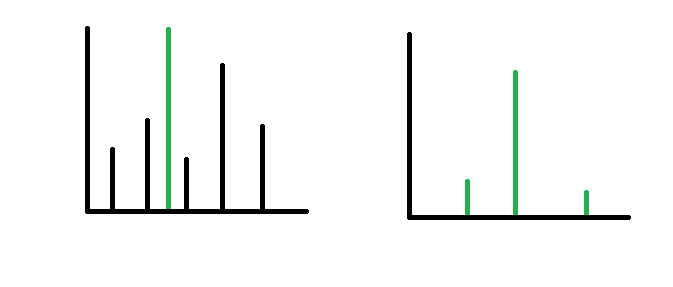
\includegraphics[width=\linewidth]{pictures/mass_spec.png}
  \caption{\textbf{Output of a proteomic mass spectrometry analysis}. The green circle represents one protein in the sample passing through the mass spectrometer}
  \label{fig:mass-spec}
\end{figure}

\subsection{Related work}
A multitude of software for analyzing bioinformatic data using containers already exist. The community-driven open source project \textit{Biocontainers} utilizes container images to create pipelines for bioinformatic applications \cite{biocontainers}. Most pipelines utilizing containers are using the software \textit{Docker} to create the containers \cite{docker}. Why Singularity containers was used in the project was due to the main benefit with using Singularity images; the images can be executed without systems administrator privileges, meaning any user can freely execute the image, such as on a HPC cluster. Non-container pipelines are a common way to analyze mass spectrometry data, such as MaxQuant and OpenMS \cite{maxquant, openms}, which were the two software compared to Quandenser-pipeline. There are Docker containers with all the components required to run OpenMS, but as explained previously, Docker containers are not suited for a shared HPC environment due to security issues \cite{openms-hpc}.

As for the software, there are a large variety of workflow managers available. KNIME is a workflow manager which aims to allow the user to visualize and connect nodes in Graphical User Interface (GUI), which was used to run a custom OpenMS pipeline as a benchmark \cite{knime}. Snakemake is a workflow manager written in python, which allows to set up pipelines in a similar way as Nextflow, without the requirement of a GUI \cite{snakemake}.
